%tag:000X
%label:"dig:exactSequencesFromCobordisms"
%type:"diagram"
%author:JeffHicks

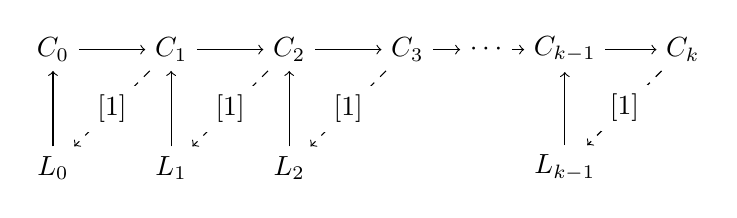
\begin{tikzpicture}




    \node (v1) at (1.5,-0.5) {$C_0$};
    \node (v2) at (3,-0.5) {$C_1$};
    \node (v3) at (4.5,-0.5) {$C_2$};
    \node (v4) at (6,-0.5) {$C_3$};
    \node (v6) at (8,-0.5) {$C_{k-1}$};
    \node (v7) at (9.5,-0.5) {$C_k$};
    \node (v8) at (1.5,-2) {$L_0$};
    \node (v9) at (3,-2) {$L_1$};
    \node (v10) at (4.5,-2) {$L_2$};
    \node (v11) at (8,-2) {$L_{k-1}$};
    \node (v5) at (7,-0.5) {$\cdots$};
    \draw[->]  (v1) edge (v2);
    \draw[->]  (v2) edge (v3);
    \draw[->]  (v3) edge (v4);
    \draw[->]  (v4) edge (v5);
    \draw[->]  (v5) edge (v6);
    \draw[->]  (v6) edge (v7);
    \draw[->]  (v8) edge (v1);
    \draw[->]  (v9) edge (v2);
    \draw[->]  (v10) edge (v3);
    \draw[->]  (v11) edge (v6);
    \draw[->,dashed]  (v2) edge  node[fill=white]{$[1]$} (v8);
    \draw[->,dashed]  (v3) edge  node[fill=white]{$[1]$} (v9);
    \draw[->,dashed]  (v4) edge  node[fill=white]{$[1]$} (v10);
    \draw[->,dashed]  (v7) edge  node[fill=white]{$[1]$}  (v11);
    \end{tikzpicture}